\chapter{One Interface, Three Bottoms}
\label{ch:overlay}

\section{The result first}

On 5~July~2026, \texttt{send\_trajectory.py} --- unchanged since the night it was written
against mock hardware --- executed its two-waypoint trajectory on the Isaac-simulated UR5e and
returned \texttt{error\_code=0}, and the sweep was confirmed \emph{visually} in the viewport.
(The return code alone is weaker than it looks --- see the tolerance lesson in this chapter's
mistakes log; the eyes were the real verifier that day.) The chapter-1
promise --- \emph{sim and real expose identical interfaces} --- is now a demonstrated property
of the stack, not a design intention. Mock was the first bottom; Isaac is the second;
September's motors are the third.

\begin{figure}[h]\centering
  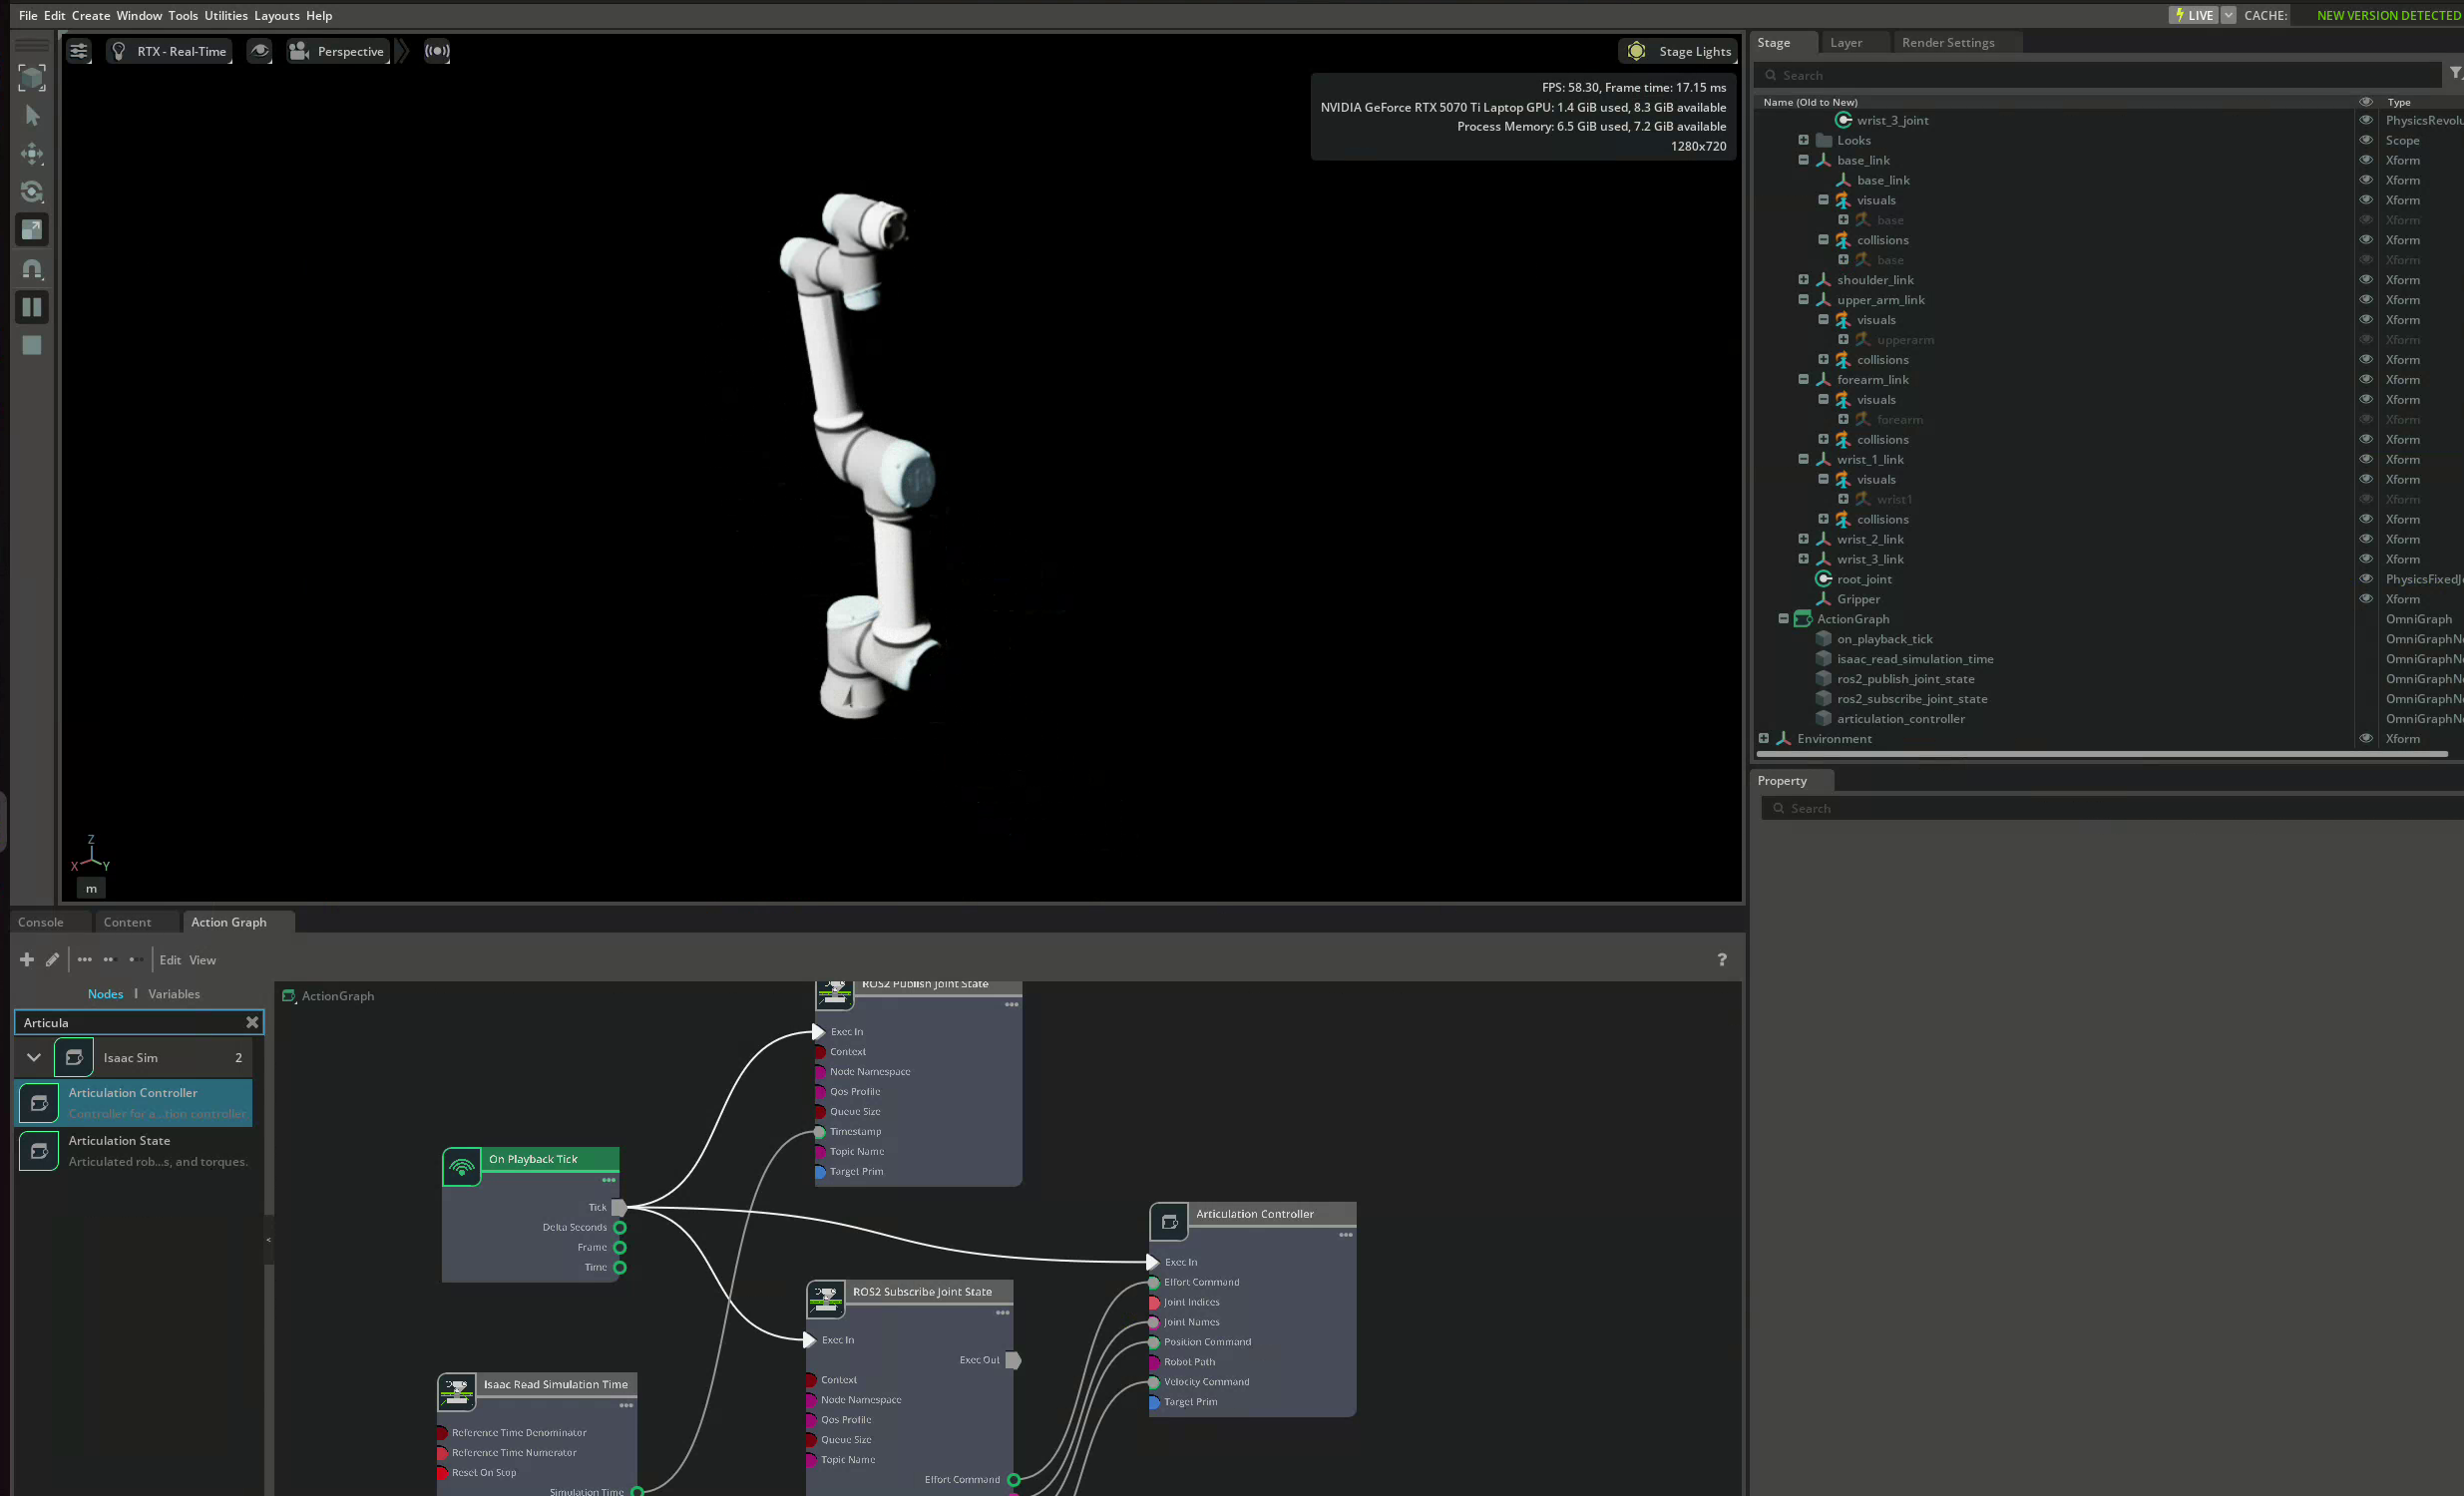
\includegraphics[width=0.95\linewidth]{figures/ch05_full_stack.png}
  \caption{The full stack mid-trajectory: PhysX viewport, the OmniGraph bridge wiring below
  (tick $\to$ publish/subscribe $\to$ articulation controller), stage tree right.}
\end{figure}

\section{The anatomy of the overlay}

Four small files (package \texttt{vanguard\_isaac\_control}) created the bridge. What each
\emph{is}, precisely:

\begin{description}
\item[\texttt{urdf/ur5e\_isaac.urdf.xacro} --- the noun.] Xacro is URDF with macros; expansion
produces one robot description with two conceptually distinct parts. The \emph{kinematic}
part (links, joints, limits) comes from UR's \texttt{ur\_robot} macro reading their config
YAMLs --- chapter~\ref{ch:fk}'s PoE chain, serialized. The \emph{\texttt{<ros2\_control>}}
part declares no geometry at all: per joint, which command/state \emph{interfaces} exist, and
which \emph{hardware plugin} provides them. Ours is
\texttt{topic\_based\_ros2\_control/TopicBasedSystem} with two parameters --- the command and
state topic names. That one block is the entire difference between the mock arm, the Isaac
arm, and the future real arm.

\item[\texttt{config/controllers.yaml} --- the loop configuration.] The controller manager
(\texttt{ros2\_control\_node}) runs read$\to$update$\to$write at 60\,Hz (matched to Isaac's
tick). The YAML names its controllers: \texttt{joint\_state\_broadcaster} (republishes
hardware state as \texttt{/joint\_states} --- which is why the Isaac-side topics were renamed
\texttt{/isaac\_*}; the plain name belongs to this broadcaster) and a
\texttt{JointTrajectoryController} deliberately \emph{instance-named}
\texttt{scaled\_joint\_trajectory\_controller} so the action path baked into
\texttt{send\_trajectory.py} resolves unchanged. Names are labels; types are behavior.

\item[\texttt{launch/isaac\_control.launch.py} --- the verb.] Starts four processes:
\texttt{robot\_state\_publisher} (live FK $\to$ TF), the controller manager (given the URDF's
control block + the YAML), and two short-lived \texttt{spawner}s that ask the manager ---
via services --- to load, configure, and activate each controller, then exit. When the manager
crashes, spawners wait forever on those services: that log signature
(\emph{``waiting for service /controller\_manager/list\_controllers''}) means \emph{look
upstream, the server died}.

\item[The data path, named end to end:] action goal $\to$ JTC spline interpolation $\to$
position commands through the hardware interface $\to$ \texttt{TopicBasedSystem} publishes
\texttt{/isaac\_joint\_commands} $\to$ Isaac's Articulation Controller drives PhysX $\to$
\texttt{/isaac\_joint\_states} at 60\,Hz $\to$ back through the plugin as controller feedback
and out as \texttt{/joint\_states} for everyone else. The script sees only the action; the
bottom is invisible by construction.
\end{description}

\section{Mistakes log}

\begin{lesson}
\textbf{A plugin is a promise someone must install.} First launch died with
\texttt{pluginlib::LibraryLoadException}: the URDF requested \texttt{TopicBasedSystem}, but
\texttt{ros-humble-topic-based-ros2-control} was never installed --- the crash log helpfully
listed every plugin that \emph{did} exist, which is the fastest way to read this failure class.
Same root pattern as the ephemeral-install lesson of chapter~\ref{ch:standin}: the
environment's source of truth is the Dockerfile, and it hadn't been rebuilt.
\end{lesson}

\begin{lesson}
\textbf{The description you include may bring its own controller.} The same crash log showed
\texttt{Loading hardware 'ur5e'} \emph{succeeding} before ours loaded: \texttt{ur\_description}
v2.10's macro generates its \emph{own} \texttt{ros2\_control} block by default
(\texttt{generate\_ros2\_control\_tag:=true}), so the robot had two hardware systems claiming
the same six joints. Fix: one attribute, \texttt{generate\_ros2\_control\_tag="false"}.
Verification habit adopted: after any description change,
\texttt{xacro ... | grep -c '<ros2\_control'} must print exactly 1.
\end{lesson}

\begin{lesson}
\textbf{One letter, zero communication.} After everything reported success, the arm did not
move: the controller published \texttt{/isaac\_joint\_commands} while Isaac subscribed to
\texttt{/isaac\_joint\_command} --- singular. Videos and stares found nothing;
\texttt{ros2 topic info} found it in one command: \texttt{pub=1, sub=0} on one topic and the
mirror image on its sibling is the exact signature of a name mismatch. Standing rule: when a
topic chain is silent, \emph{count the endpoints before watching the robot}.
\end{lesson}

\begin{lesson}
\textbf{``Success'' is only as strong as its tolerances (a correction).} This chapter first
claimed \texttt{error\_code=0} proved PhysX tracked the trajectory within tolerance. Wrong ---
and the proof was an accident: a leftover experiment value (elbow $=4.0$\,rad, past its limit)
also returned success. Humble's \texttt{JointTrajectoryController} checks goal tolerances only
if the YAML configures \texttt{constraints}; ours didn't, so success meant ``trajectory sent,''
not ``arm arrived.'' PhysX clamped the impossible joint; nobody objected. Fix queued: explicit
\texttt{constraints} per joint, after which \texttt{error\_code=0} becomes an instrument
reading instead of a pleasantry. Meta-lesson for the book itself: claims about what a check
certifies must be verified against the check's configuration, not its name.
\end{lesson}

\begin{lesson}
\textbf{A trailing space after a backslash is invisible and fatal.} The Dockerfile's line
continuation \texttt{ros-humble-ur-robot-driver \textbackslash\textvisiblespace} (note the
space \emph{after} the backslash) breaks the multi-line \texttt{RUN} --- the next line becomes
a separate, invalid instruction. Found in review before it cost a build. Editors with
show-whitespace would have flagged it; ours now does.
\end{lesson}

\section{Phase 0b: closed}

Remaining Phase-0 work builds \emph{on} this bridge rather than extending it: the IDMO panel
scene in Isaac, MoveIt pointed at the overlay stack, the six skill stubs, teleop, and the
LeRobot recording path for P1. The interface layer itself is done --- and it is the most
load-bearing thing this project will ever build, which is why it got five chapters.
